\documentclass[a4paper, 12pt]{book}
%\documentclass[a4paper, 12pt, draft]{book}  Nalogo preverite tudi z opcijo draft, ki vam bo pokazala, katere vrstice so predolge!



\usepackage[utf8x]{inputenc}   % omogoča uporabo slovenskih črk kodiranih v formatu UTF-8
\usepackage[slovene,english]{babel}    % naloži, med drugim, slovenske delilne vzorce
\usepackage[pdftex]{graphicx}  % omogoča vlaganje slik različnih formatov
\usepackage{fancyhdr}          % poskrbi, na primer, za glave strani
\usepackage{amssymb}           % dodatni simboli
\usepackage{amsmath}           % eqref, npr.
\usepackage[hyphens]{url}  % dodal Solina
\usepackage{comment}       % dodal Solina

\usepackage[pdftex, colorlinks=true,
						citecolor=black, filecolor=black, 
						linkcolor=black, urlcolor=black,
						pagebackref=false, 
						pdfproducer={LaTeX}, pdfcreator={LaTeX}, hidelinks]{hyperref}

\usepackage{color}       % dodal Solina
\usepackage{soul}       % dodal Solina

%%%%%%%%%%%%%%%%%%%%%%%%%%%%%%%%%%%%%%%%
%	DIPLOMA INFO
%%%%%%%%%%%%%%%%%%%%%%%%%%%%%%%%%%%%%%%%
\newcommand{\ttitle}{Mobilna aplikacija Asana Master}
\newcommand{\ttitleEn}{Mobile app Asana Master}
\newcommand{\tsubject}{\ttitle}
\newcommand{\tsubjectEn}{\ttitleEn}
\newcommand{\tauthor}{Klementina Garbajs}
\newcommand{\tkeywords}{Joga, Mobilna aplikacija}
\newcommand{\tkeywordsEn}{Yoga, Mobile app}


%%%%%%%%%%%%%%%%%%%%%%%%%%%%%%%%%%%%%%%%
%	HYPERREF SETUP
%%%%%%%%%%%%%%%%%%%%%%%%%%%%%%%%%%%%%%%%
\hypersetup{pdftitle={\ttitle}}
\hypersetup{pdfsubject=\ttitleEn}
\hypersetup{pdfauthor={\tauthor, kg4597@student.uni-lj.si}}
\hypersetup{pdfkeywords=\tkeywordsEn}

%%%%%%%%%%%%%%%%%%%%%%%%%%%%%%%%%%%%%%%%
% postavitev strani
%%%%%%%%%%%%%%%%%%%%%%%%%%%%%%%%%%%%%%%%  

\addtolength{\marginparwidth}{-20pt} % robovi za tisk
\addtolength{\oddsidemargin}{40pt}
\addtolength{\evensidemargin}{-40pt}

\renewcommand{\baselinestretch}{1.3} % ustrezen razmik med vrsticami
\setlength{\headheight}{15pt}        % potreben prostor na vrhu
\renewcommand{\chaptermark}[1]%
{\markboth{\MakeUppercase{\thechapter.\ #1}}{}} \renewcommand{\sectionmark}[1]%
{\markright{\MakeUppercase{\thesection.\ #1}}} \renewcommand{\headrulewidth}{0.5pt} \renewcommand{\footrulewidth}{0pt}
\fancyhf{}
\fancyhead[LE,RO]{\sl \thepage}
\fancyhead[RE]{\sc \tauthor}              % dodal Solina
\fancyhead[LO]{\sc Diplomska naloga}     % dodal Solina


\newcommand{\BibTeX}{{\sc Bib}\TeX}

%%%%%%%%%%%%%%%%%%%%%%%%%%%%%%%%%%%%%%%%
% naslovi
%%%%%%%%%%%%%%%%%%%%%%%%%%%%%%%%%%%%%%%%  


\newcommand{\autfont}{\Large}
\newcommand{\titfont}{\LARGE\bf}
\newcommand{\clearemptydoublepage}{\newpage{\pagestyle{empty}\cleardoublepage}}
\setcounter{tocdepth}{1}	      % globina kazala

%%%%%%%%%%%%%%%%%%%%%%%%%%%%%%%%%%%%%%%%
% konstrukti
%%%%%%%%%%%%%%%%%%%%%%%%%%%%%%%%%%%%%%%%  
\newtheorem{izrek}{Izrek}[chapter]
\newtheorem{trditev}{Trditev}[izrek]
\newenvironment{dokaz}{\emph{Dokaz.}\ }{\hspace{\fill}{$\Box$}}

%%%%%%%%%%%%%%%%%%%%%%%%%%%%%%%%%%%%%%%%%%%%%%%%%%%%%%%%%%%%%%%%%%%%%%%%%%%%%%%
%% PDF-A
%%%%%%%%%%%%%%%%%%%%%%%%%%%%%%%%%%%%%%%%%%%%%%%%%%%%%%%%%%%%%%%%%%%%%%%%%%%%%%%


%%%%%%%%%%%%%%%%%%%%%%%%%%%%%%%%%%%%%%%% 
% define medatata
%%%%%%%%%%%%%%%%%%%%%%%%%%%%%%%%%%%%%%%% 
\def\Title{\ttitle}
\def\Author{\tauthor, kg4597@student.uni-lj.si}
\def\Subject{\ttitleEn}
\def\Keywords{\tkeywordsEn}

%%%%%%%%%%%%%%%%%%%%%%%%%%%%%%%%%%%%%%%% 
% \convertDate converts D:20080419103507+02'00' to 2008-04-19T10:35:07+02:00
%%%%%%%%%%%%%%%%%%%%%%%%%%%%%%%%%%%%%%%% 
\def\convertDate{%
    \getYear
}

{\catcode`\D=12
 \gdef\getYear D:#1#2#3#4{\edef\xYear{#1#2#3#4}\getMonth}
}
\def\getMonth#1#2{\edef\xMonth{#1#2}\getDay}
\def\getDay#1#2{\edef\xDay{#1#2}\getHour}
\def\getHour#1#2{\edef\xHour{#1#2}\getMin}
\def\getMin#1#2{\edef\xMin{#1#2}\getSec}
\def\getSec#1#2{\edef\xSec{#1#2}\getTZh}
\def\getTZh +#1#2{\edef\xTZh{#1#2}\getTZm}
\def\getTZm '#1#2'{%
    \edef\xTZm{#1#2}%
    \edef\convDate{\xYear-\xMonth-\xDay T\xHour:\xMin:\xSec+\xTZh:\xTZm}%
}

\expandafter\convertDate\pdfcreationdate 

%%%%%%%%%%%%%%%%%%%%%%%%%%%%%%%%%%%%%%%%
% get pdftex version string
%%%%%%%%%%%%%%%%%%%%%%%%%%%%%%%%%%%%%%%% 
\newcount\countA
\countA=\pdftexversion
\advance \countA by -100
\def\pdftexVersionStr{pdfTeX-1.\the\countA.\pdftexrevision}


%%%%%%%%%%%%%%%%%%%%%%%%%%%%%%%%%%%%%%%%
% XMP data
%%%%%%%%%%%%%%%%%%%%%%%%%%%%%%%%%%%%%%%%  
\usepackage{xmpincl}
\includexmp{pdfa-1b}

%%%%%%%%%%%%%%%%%%%%%%%%%%%%%%%%%%%%%%%%
% pdfInfo
%%%%%%%%%%%%%%%%%%%%%%%%%%%%%%%%%%%%%%%%  
\pdfinfo{%
    /Title    (\ttitle)
    /Author   (\tauthor, kg4597@student.uni-lj.si)
    /Subject  (\ttitleEn)
    /Keywords (\tkeywordsEn)
    /ModDate  (\pdfcreationdate)
    /Trapped  /False
}


%%%%%%%%%%%%%%%%%%%%%%%%%%%%%%%%%%%%%%%%%%%%%%%%%%%%%%%%%%%%%%%%%%%%%%%%%%%%%%%
%%%%%%%%%%%%%%%%%%%%%%%%%%%%%%%%%%%%%%%%%%%%%%%%%%%%%%%%%%%%%%%%%%%%%%%%%%%%%%%

\begin{document}
\selectlanguage{slovene}
\frontmatter
\setcounter{page}{1} %
\renewcommand{\thepage}{}       % preprecimo težave s številkami strani v kazalu
\newcommand{\sn}[1]{"`#1"'}                    % dodal Solina (slovenski narekovaji)

%%%%%%%%%%%%%%%%%%%%%%%%%%%%%%%%%%%%%%%%
%naslovnica
 \thispagestyle{empty}%
   \begin{center}
    {\large\sc Univerza v Ljubljani\\%
      Fakulteta za računalništvo in informatiko}%
    \vskip 10em%
    {\autfont \tauthor\par}%
    {\titfont \ttitle \par}%
    {\vskip 3em \textsc{DIPLOMSKO DELO\\[5mm]         % dodal Solina za ostale študijske programe
%    VISOKOŠOLSKI STROKOVNI ŠTUDIJSKI PROGRAM\\ PRVE STOPNJE\\ RAČUNALNIŠTVO IN INFORMATIKA}\par}%
    UNIVERZITETNI  ŠTUDIJSKI PROGRAM\\ PRVE STOPNJE\\ RAČUNALNIŠTVO IN INFORMATIKA}\par}%
%    INTERDISCIPLINARNI UNIVERZITETNI\\ ŠTUDIJSKI PROGRAM PRVE STOPNJE\\ RAČUNALNIŠTVO IN MATEMATIKA}\par}%
%    INTERDISCIPLINARNI UNIVERZITETNI\\ ŠTUDIJSKI PROGRAM PRVE STOPNJE\\ UPRAVNA INFORMATIKA}\par}%
%    INTERDISCIPLINARNI UNIVERZITETNI\\ ŠTUDIJSKI PROGRAM PRVE STOPNJE\\ MULTIMEDIJA}\par}%
    \vfill\null%
    {\large \textsc{Mentor}: doc.\ dr.  Mira Trebar\par}%
    {\vskip 2em \large Ljubljana, 2021 \par}%
\end{center}
% prazna stran
%\clearemptydoublepage      % dodal Solina (izjava o licencah itd. se izpiše na hrbtni strani naslovnice)

%%%%%%%%%%%%%%%%%%%%%%%%%%%%%%%%%%%%%%%%
%copyright stran
\thispagestyle{empty}
\vspace*{8cm}

\noindent
{\sc Copyright}. 
Rezultati diplomske naloge so intelektualna lastnina avtorja in Fakultete za računalništvo in informatiko Univerze v Ljubljani.
Za objavo in koriščenje rezultatov diplomske naloge je potrebno pisno privoljenje avtorja, Fakultete za računalništvo in informatiko ter mentorja.

\begin{center}
\mbox{}\vfill
\emph{Besedilo je oblikovano z urejevalnikom besedil \LaTeX.}
\end{center}
% prazna stran
\clearemptydoublepage

%%%%%%%%%%%%%%%%%%%%%%%%%%%%%%%%%%%%%%%%
% stran 3 med uvodnimi listi
\thispagestyle{empty}
\vspace*{4cm}

\noindent
Fakulteta za računalništvo in informatiko izdaja naslednjo nalogo:
\medskip
\begin{tabbing}
\hspace{32mm}\= \hspace{6cm} \= \kill

Tematika naloge:
\end{tabbing}
Besedilo teme diplomskega dela študent prepiše iz študijskega informacijskega sistema, kamor ga je vnesel mentor. V nekaj stavkih bo opisal, kaj pričakuje od kandidatovega diplomskega dela. Kaj so cilji, kakšne metode uporabiti, morda bo zapisal tudi ključno literaturo.
\vspace{15mm}

\vspace{2cm}

% prazna stran
\clearemptydoublepage

% zahvala
\thispagestyle{empty}\mbox{}\vfill\null\it%
\noindent
Na tem mestu zapišite, komu se zahvaljujete za izdelavo diplomske naloge. Pazite, da ne boste koga pozabili. Utegnil vam bo zameriti. Temu se da izogniti tako, da celotno zahvalo izpustite.
\rm\normalfont

% prazna stran
\clearemptydoublepage

%%%%%%%%%%%%%%%%%%%%%%%%%%%%%%%%%%%%%%%%
% kazalo
\pagestyle{empty}
\def\thepage{}% preprecimo tezave s stevilkami strani v kazalu
\tableofcontents{}

% prazna stran
\clearemptydoublepage

%%%%%%%%%%%%%%%%%%%%%%%%%%%%%%%%%%%%%%%%
% seznam kratic

\chapter*{Seznam uporabljenih kratic}  % spremenil Solina, da predolge vrstice ne gredo preko desnega roba

\noindent\begin{tabular}{p{0.1\textwidth}|p{.4\textwidth}|p{.4\textwidth}}    % po potrebi razširi prvo kolono tabele na račun drugih dveh!
  {\bf kratica} & {\bf angleško} & {\bf slovensko} \\ \hline
  {\bf IDE} & {\bf integrated development enviroment} & {\bf integrirano razvojno okolje} \\ \hline
  {\bf } & \\
  {\bf } & \\
  {\bf } & \\
%  \dots & \dots & \dots \\
\end{tabular}


% prazna stran
\clearemptydoublepage

%%%%%%%%%%%%%%%%%%%%%%%%%%%%%%%%%%%%%%%%
% povzetek
\addcontentsline{toc}{chapter}{Povzetek}
\chapter*{Povzetek}

\noindent\textbf{Naslov:} \ttitle
\bigskip

\noindent\textbf{Avtor:} \tauthor
\bigskip

%\noindent\textbf{Povzetek:} 
\noindent 
Za diplomsko delo sem se odločila razviti mobilno aplikacijo Asana Master, ki bi v neki celoti zaobjela potovanje posameznika po njegovi poti Joge. Asane oz. položaji imajo v Jogi velik pomen, zato je pomembno, da je izvajanje le teh pravilno in v skladu z zmožnostmi posameznika. Prav z namenom učenja pravilne izvedbe položajev, spremljanjem napredka in sledenja lastnim občutkom praktikantov, pa sem razvila aplikacijo, ki je primerna tako za začetne kot nadaljevalne praktikante, saj so Asane razdeljene na različne stopnje, prav tako pa si praktikant lahko sam določi svoje cilje. 

\bigskip

\noindent\textbf{Ključne besede:} \tkeywords.
% prazna stran
\clearemptydoublepage

%%%%%%%%%%%%%%%%%%%%%%%%%%%%%%%%%%%%%%%%
% abstract
\selectlanguage{english}
\addcontentsline{toc}{chapter}{Abstract}
\chapter*{Abstract}

\noindent\textbf{Title:} \ttitleEn
\bigskip

\noindent\textbf{Author:} \tauthor
\bigskip

%\noindent\textbf{Abstract:} 
\noindent 
For my dissertation, I decided to develop the Asana Master mobile app, which would completely encompass an individual's journey along his Yoga path. Asanas or positions are of great part in Yoga, so it is important that the implementation of these is correct and in accordance with the abilities of the individual. In order to learn how to perform the positions correctly, monitor progress and follow the practitioners' own feelings, I developed an application that is suitable for both beginners and advanced practitioners, as Asanas are divided into different levels, and the practitioner can set his own goals.
\bigskip

\noindent\textbf{Keywords:} \tkeywordsEn.
\selectlanguage{slovene}
% prazna stran
\clearemptydoublepage

%%%%%%%%%%%%%%%%%%%%%%%%%%%%%%%%%%%%%%%%
\mainmatter
\setcounter{page}{1}
\pagestyle{fancy}

\chapter{Uvod}
Joga je za nekoga lahko le oblika sprostitve, način napajanja z energijo, vadba za boljše počutje, za tiste, ki se z jogo ukvarjajo bolj intenzivno, pa je joga predvsem izjemno, do potankosti izdelano in premišljeno urjenje osebnosti, ki lahko človeku omogoči, da dozori. Joga je pot k sebi. Nima pa joga le pozitivnih učinkov na um, temveč seveda tudi na telo. 
Z leti postane naše telo manj gibčno, utrujeno, bolj občutljivo in nagnjeno k poškodbam, kar pa lahko učinkovito odpravimo z vadbo joge, saj telo postane prožnejše, bolj gibljivo in močnejše. Joga so telesni položaji ali asane preko katerih začutimo in spoznavamo svoje telo, ga nadzorujemo in izboljšujemo, vendar praksa asan ne sme biti brezglava in pretirana, zato je poznavanje joga položajev in pravilne izvedbe le-teh zelo pomembno. 
In kaj je asana? Sanskrtski izraz asana pomeni poza ali položaj telesa. Asana je psiho-somatska jogiska vaja za telo in um, saj z njo vplivamo tako na počutje telesa, kot tudi uma. Pozorni moramo biti tako na pravilen položaj telesa, kot tudi na naše dihanje. 

Prav z namenom pravilnega izvajanja položajev in spremljanjem napredka pri tem, pa sem se za svojo diplomsko nalogo odločila razviti mobilno aplikacijo, ki bi bodočim joga učiteljem in tudi vsem ostalim praktikantom joge omogočala lažje in bolj zabavno obliko učenja, ter dodatno motivacijo za napredek. Aplikacijo sem razvila z uporabo ogrodja React Native in odprtokodno platformo Expo. Za pisanje kode sem uporabila jezike, Java Script, TypeScript in SQL. Aplikacija teče na Expotovem lokalnem strežniku, za povezavo do baze podatkov pa je uporabljen strežnik Express. Podatki so shranjeni v MySql bazi, ki teče preko lokalnega MySQL strežnika.

\chapter{Joga}
\label{ch0}

\section{Zgodovina joge}

\textbf{Kaj je joga in njeno bistvo?}\\

Joga združuje načine zavedanja, zaznavanja, doživljanja, soočanja, spoznavanja in delovanja, preko katerih je človek zmožen bivati neodvisno od lastne pogojenosti. V jogijskih spisih je ta zmožnost bivanja opisana kot stanje odrešitve, saj je preko nje človek odrešen trpljenja kateremu je podvržen kot človeško bitje bivajoče v tem svetu. Joga namreč izhaja iz spoznanja, da trpljenje ni neločljivo povezano s človeškim bitjem oziroma ni neizogibno vsebovano v svetu v katerem živi. Trpljenje je šele učinek nezmožnosti delovati na določen način. Beseda joga izhaja iz korena besede yuj, kar pomeni povezovati. Joga povezuje snovnost in duhovnost, telo in duha. Medsebojno so-delovanje telesa in duha povezuje v usklajeno, dopolnjujoče se gibanje. Če želi človek povezati svoje telo in duha na omenjeni način, se mora biti najprej zmožen razvezati oziroma oddaljiti od lastnih določujočih pogojev.~\cite{oJogi}\\ 

Kot posebna metoda preseganja človeške pogojenosti, je omenjena že v starodavnih vedskih spisih katerih nastanke zgodovinarji umeščajo na območje današnja Indije. Preden se je namreč razširila kot uveljavljena praksa so kot prevladujoči načini samo-preseganja služili predvsem obredni rituali žrtvovanja. Preko ritualov žrtvovanja, ki so vsebovali elemente smrti in ponovnega rojstva, so si ljudje poskušali zagotoviti moč nadzora nad lastno minljivostjo. 

V obdobju prvih upanišadskih spisov so obredni rituali začeli izgubljati svoj vlogo prevladujočega načina samo-preseganja. Zmožnost odrešitve je prenehala obstajati kot poseben privilegij pogojen s poznavanjem ritualnih praks, saj se je iz rituala, kot sredstva odrešitve, pozornost preusmerila na osebo in način njenega bivanja. Modreci ršiji - avtorji upanišadskih spisov - so namreč v svojih nazorih poudarjali, da je odrešitev zmožen doseči prav vsak z načinom svojega bivanja in delovanja.

To bivanje in delovanje so opisali v filozofskih nazorih samkhye iz katerih izhaja tudi filozofija joge. Filozofija samkhye temelji na predpostavki, da je človeško trpljenje posledica nepoznavanja samega sebe in vzrokov svojih dejanj. Sprememba načina bivanja, ki bi onemogočila trpljenje je pogojena spoznanjem in udejanjanjem samega sebe. To spoznanje ni razumsko spoznanje, saj spoznavajoči ne ustvarja spoznanja, ki bi bilo ločeno od njega, ampak je spoznanje oziroma se (sam sebi) razodeva kot spoznanje.

Spoznanje samega sebe se razodeva na nivoju skupne zavesti. Tu se jaz zaveda samega sebe neodvisno od fizičnega in psihičnega doživljanja. S tem, ko je zmožen kot pričujoča zavest bivati onstran fizičnega in psihičnega izkustva, lahko spoznava in spreminja pogoje lastnega bivanja in vzroke svojega delovanja. \\

Filozofija joge je prevzela osnovne predpostavke samkhye, le da odrešitve ne povezuje toliko s spoznanjem, kolikor z načinom delovanja. Človek je zmožen preseči lastno pogojenost in bivati neodvisno od materialnega sveta (za katerega se je predpostavljajo, da vsebuje tako fizično kot psihično realnost) prav z določenim načinom doživljanja in delovanja v materialnem svetu.

Omenjen način doživljanja in delovanja je v filozofiji joge opisan kot jogijska praksa. \\ 
Prvo sistematično zbirko jogijskih praks, ki so se izvajale na območju današnje Indije je izdelal Patanjali v svojih Yoga-sutrah (njegovo življenje zgodovinarji umeščajo v obdobje od 2. stol. pr. n. št - 5. st. n. št.). V njih izpostavlja, kako praksa joge ne omogoča zgolj duhovne neodvisnosti od pogojev materialnega sveta, ampak tudi zmožnost njihovega spreminjanja. S pomočjo prakse joge, ki vključuje tako fizično, psihično kot duhovno komponento, smo zmožni spreminjati svojo nezavedno pogojenost in iz nje izhajajočo zmožnost delovanja.~\cite{ZgodovinaJoge}

Tradicionalno jogo sestavlja osem temeljnih vej (ash – osem, anga – veja), ki jih je prvič sistematično opisal Patanjali v svojih Yoga-sutrah:

\begin{enumerate}
	\item \textbf{Yama ali etične zmožnosti} 
		\begin{itemize}
			\item nenasilje (ahimsa) – nezmožnost škodovati sebi in drugim
			\item resnicoljubnost (satya) – usklajenost govora z dejanji
			\item onemogočanje kraje oziroma težnje po prilaščanju tega kar nam ne pripada (asteya)
			\item neodvisnost od spolnih potreb (brahmacarya)
			\item onemogočenje pohlepa (aparigraha) oziroma težnje po prilaščanju tega česar ne potrebujemo
		\end{itemize}
	
	\item \textbf{Niyama ali discipline}
		\begin{itemize}
			\item čiščenje telesa in duha (sauca)
			\item zmožnost izkusiti zadovoljstvo neodvisno od zunanjih dejavnikov (samtosa)
			\item askeza (tapas)
			\item odsotnost besed (kastha mauna)
			\item odsotnost gest in kretenj (akara mauna)
			\item študij načinov samo-preseganja
		\end{itemize}

	\item \textbf{Asana ali telesni položaji}
	\item \textbf{Pranayama ali dihalne tehnike}
	\item \textbf{Pratyahara ali neodvisnost čutil od zaznavanja zunanjih dejavnikov}
	\item \textbf{Dharana ali zbranost in zmožnost nadzorovanega usmerjanja pozornosti}
	\item \textbf{Dhyana ali meditacija}
	\item \textbf{Samadhi ali stanje skupne zavesti}
\end{enumerate}


\section{Asane in njihov pomen}
Beseda asana pomeni stabilen in udoben položaj. Največkrat pa jo v slovenščini enačimo s terminom vaja ali položaj.\\ 

V hatha jogi so asane ena osnovnih tehnik telesnega gibanja. Asane dajejo telesu gibljivost in pravilno držo, ki omogoča optimalno energetsko in telesno stabilnost, usmerjene so v živčni sistem, predvsem v hrbtenico, ki je po jogijski anatomiji osnovna energetska os našega bivanja.

Začetniki v hatha jogi so se morali najprej naučiti, kako pravilno stati, sedeti in ležati. Zato se jogijska praksa tudi bistveno razlikuje od vseh drugih vadb, saj zahteva poleg natančnega, pravilnega izvajanja asan tudi pozornost, usmerjenost uma v to, kar počnemo. V asani smo, kot pove že sanskrtsko ime "as" oz. biti, tukaj in zdaj.

Asan je nešteto, nekateri viri navajajo številko 70.–80.000. Poimenovali so jih po živalih, rastlinah, mineralih in  božanstvih. Bilo naj bi jih toliko, kolikor je oblik življenja na zemlji. Večina asan vsebuje hatha princip, ki pomeni princip moči. Zelo pomembno je, da asane izvajamo primerno svojim telesnim sposobnostim in pravilno, kar pomeni postopnost učenja in poslušanje svojega telesa. Nikoli ne izvajamo asan preko svojih zmožnosti, ampak le do praga bolečine. \\ 

Izvedba asane naj bi bila stabilna in hkrati selektivno sproščena. Dihanje je sproščeno, enakomerno, pozornost je usmerjena v počutje telesa, opazujemo sporočila telesa, umirimo um in zadržujemo položaj toliko časa, dokler čutimo asano v vseh navedenih lastnostih. 

Skozi asane se nam razkrivajo naši ustaljeni psihofizični vzorci, ki jih običajno doživimo kot omejitve. V jogi ni tekmovalnosti, vsak je v svoji asani, ki trenutno ustreza njegovemu psihofizičnemu stanju. Učitelji joge pogosto pravijo, da je tista asana, ki nam je najmanj všeč, pravzaprav naša asana.

Z rednim in discipliniranim izvajanjem asan se prožnost telesa izredno poveča. Mnoge asane učinkujejo tudi terapevtsko in lahko odpravijo težave, ki nas pestijo dolgo časa in so morda videti nerešljive, odpravi pa jih lahko že pravilna drža telesa. Hkrati se poveča tudi naša prožnost duha: opazimo lahko spremembe v svojem dojemanju sveta, samozavesti, odprtosti, sposobnosti, da ocenimo položaj in ugotovimo, kaj je bistvo in kaj nepomembna navlaka. Trdno stojimo na tleh, z odprtim srcem in notranjo radostjo, ki ne potrebuje zunanjih dražljajev. Takrat smo prestopili prvo, pomembno stopnico na poti joge.~\cite{Asane} \\

Bistvo izvajanja asane ni nujno v popolni izvedbi. Bistvo asane je v popolnem medsebojnem zavedanju duše in telesa.


\chapter{Opis aplikacije}
\label{ch1}

\section{Ideja in zasnova aplikacije}

Živimo v svetu, kjer je imeti veliko mobilnih aplikacij nekaj običajnega, saj za vsako aktivnost, ki si jo izmislimo, obstaja mobilna aplikacija. A ko se želiš nekaj naučiti oz. v nečem izboljšati, ti lahko ravno prevelik nabor različnih aplikacij predstavlja oviro. V kolikor morda nisi najbolj organiziran človek, ti lahko možnost izbire ustvari še večjo zmedo. Prav iz tega razloga, se je rodila ideja o aplikaciji Asana Master, kjer ima uporabnik zgolj z eno aplikacijo možnost učenja o različnih položajih v jogi, možnost spremljanja programa za izboljšanje gibčnosti, inverzij itd., prav tako pa ima možnost ob tem še spremljati svoj lasten napredek in izraziti svoje občutke. Torej vse zapakirano na enem mestu. 

Razvoj mobilnih aplikacij ne bi smel biti več tako osredotočen le na eno glavno funkcionalnost, saj počasi prihaja čas, ko smo ljudje vedno bolj zasičeni z različnimi podatki, aplikacijami in načini shranjevanja, zato se bomo vedno bolj nagibali k aplikacijam, ki omogočajo več funkcionalnosti v enem.

\section{Načrtovanje aplikacije in zbiranje podatkov}

Načrtovanje aplikacije se je začelo s prototipom uporabniškega vmesnika mobilne aplikacije, saj je oblikovanje uporabniškega vmesnika pomemben sestavni del oblikovanja uporabniške izkušnje. Pri oblikovanju mobilne aplikacije se je pomembno usmeriti tako na estetiko kot seveda, tudi na funkcionalnost aplikacije. Vmesnik smo poskusili narediti čim bolj pregleden in enostaven za uporabo. Prav s tem namenom je v aplikacijo dodanih kar nekaj slik in tudi videoposnetkov. 

Prototip smo izdelali s pomočjo spletne platforme za izdelavo prototipov Proto.io, (Slika~\ref{protoio}). Izdelani so bili nekateri ključni zasloni aplikacije, glavne funkcionalnosti aplikacije, povezave med njimi in oblikovano glavno ozadje aplikacije na začetnem prijavnem zaslonu, ter ostali gradniki aplikacije.\\

\begin{figure}[htbp]
\begin{center}
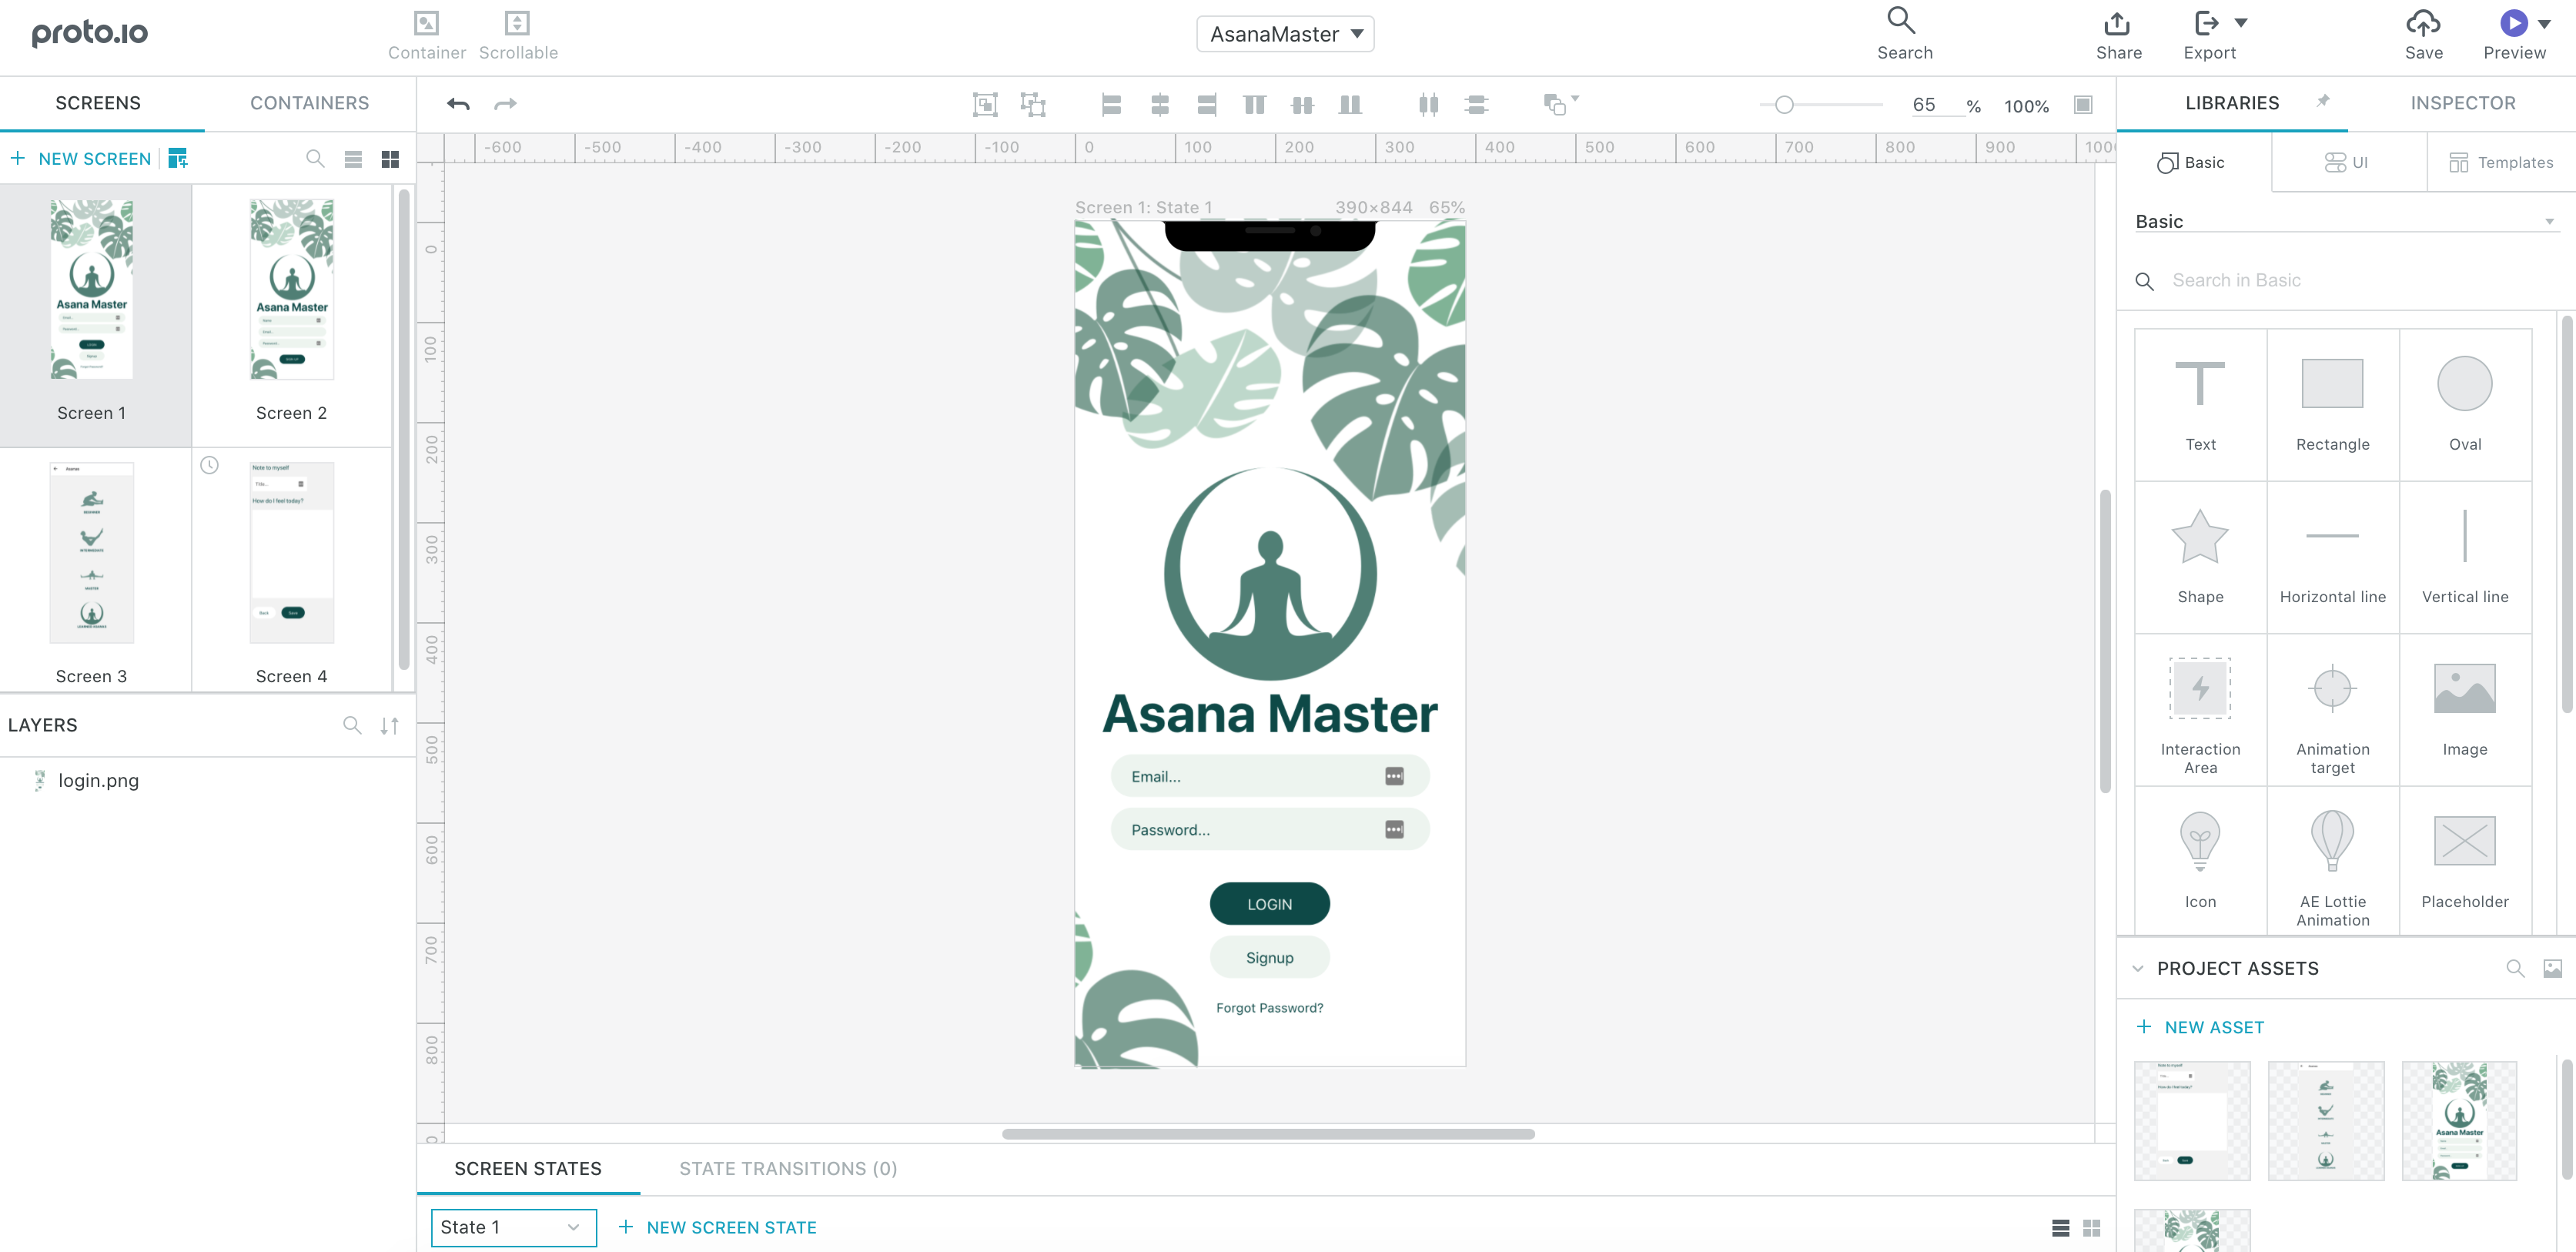
\includegraphics[scale=.23]{protoio.jpg}
\end{center}
\caption{Spletna platforma za ustvarjanje prototipov, Protoio.}
\label{protoio}
\end{figure}

Izdelavi prototipa je sledila raziskava tehnologij in primernih orodij za sam razvoj mobilne aplikacije, pri čemer je prišlo predvsem do primerjave različnih orodij za izdelavo mobilne aplikacije. Primerjali smo integrirano razvojno okolje (angl. integrated development environment, IDE) za razvoj aplikacij za operacijski sistem Android, ter razvojnim okoljem Expo, ki z uporabo React Native platforme in orodij, omogoča razvoj tako spletnih, kot mobilnih aplikacij na operacijskem sistemu Android in iOS. Zaradi možnosti razvoja na obeh operacijskih sistemih, smo prišli do zaključka, da bomo za razvoj aplikacije uporabili Expo.\\

Po začetnem načrtovanju izdelave smo se nato lotili še zbiranja podatkov o jogi in položajih v jogi. Podatki o jogi in položajih so vzeti iz knjige The Top 100 Best Yoga Poses Relieve Stress, Increase Flexibility, and Gain Strength, avtorice Susan Hollister~\cite{yoga}. Vir nekaterih slik je tudi zgoraj omenjena knjiga, nekatere pa smo pridobili preko spletne strani Verywellfit~\cite{verywellfit}. Videoposnetki, ki uporabnikom omogočajo izboljšanje položajev in napredovanja, pa so predvajani preko platforme, za deljenje videoposnetkov, Youtube.

\section{Glavne funkcionalnosti in delovanje aplikacije}
Ob zagonu mobilne aplikacije uporabnik najprej pride na stran za prijavo, (Slika~\ref{prijava}, ~\ref{registracija}). V kolikor uporabnik še ni registriran, mora najprej opraviti registracijo, s klikom na gumb Sign in, kar ga preusmeri na stran za registracijo. Za uspešno registracijo mora vnesti svoje ali poljubno ime, svoj elektronski naslov in geslo, ki ga bo uporabljal za prijavo. V kolikor je uporabnik že registriran, a je pozabil svoje geslo, si lahko preko klika na gumb Forgot password?, na svoj elektronski naslov, pošlje povezavo za ponastavitev gesla. Po uspešni prijavi preko enega izmed zgoraj omenjenih načinov je uporabnik preusmerjen v jedro aplikacije. Ob prvi prijavi, uporabnika ob vstopu v aplikacijo pozdravi kratek uvod v aplikacijo, kjer se seznani s pojmom joga in s kratkim opisom bistva aplikacije. Po zaključenem uvodu v aplikacijo je uporabnik nato preusmerjen v glavni meni, ki je razdeljen na 3 glavne podmenije: Asanas, Goals in Notes.

\begin{figure}[!tbp]
  \centering
  \begin{minipage}[b]{0.34\textwidth}
    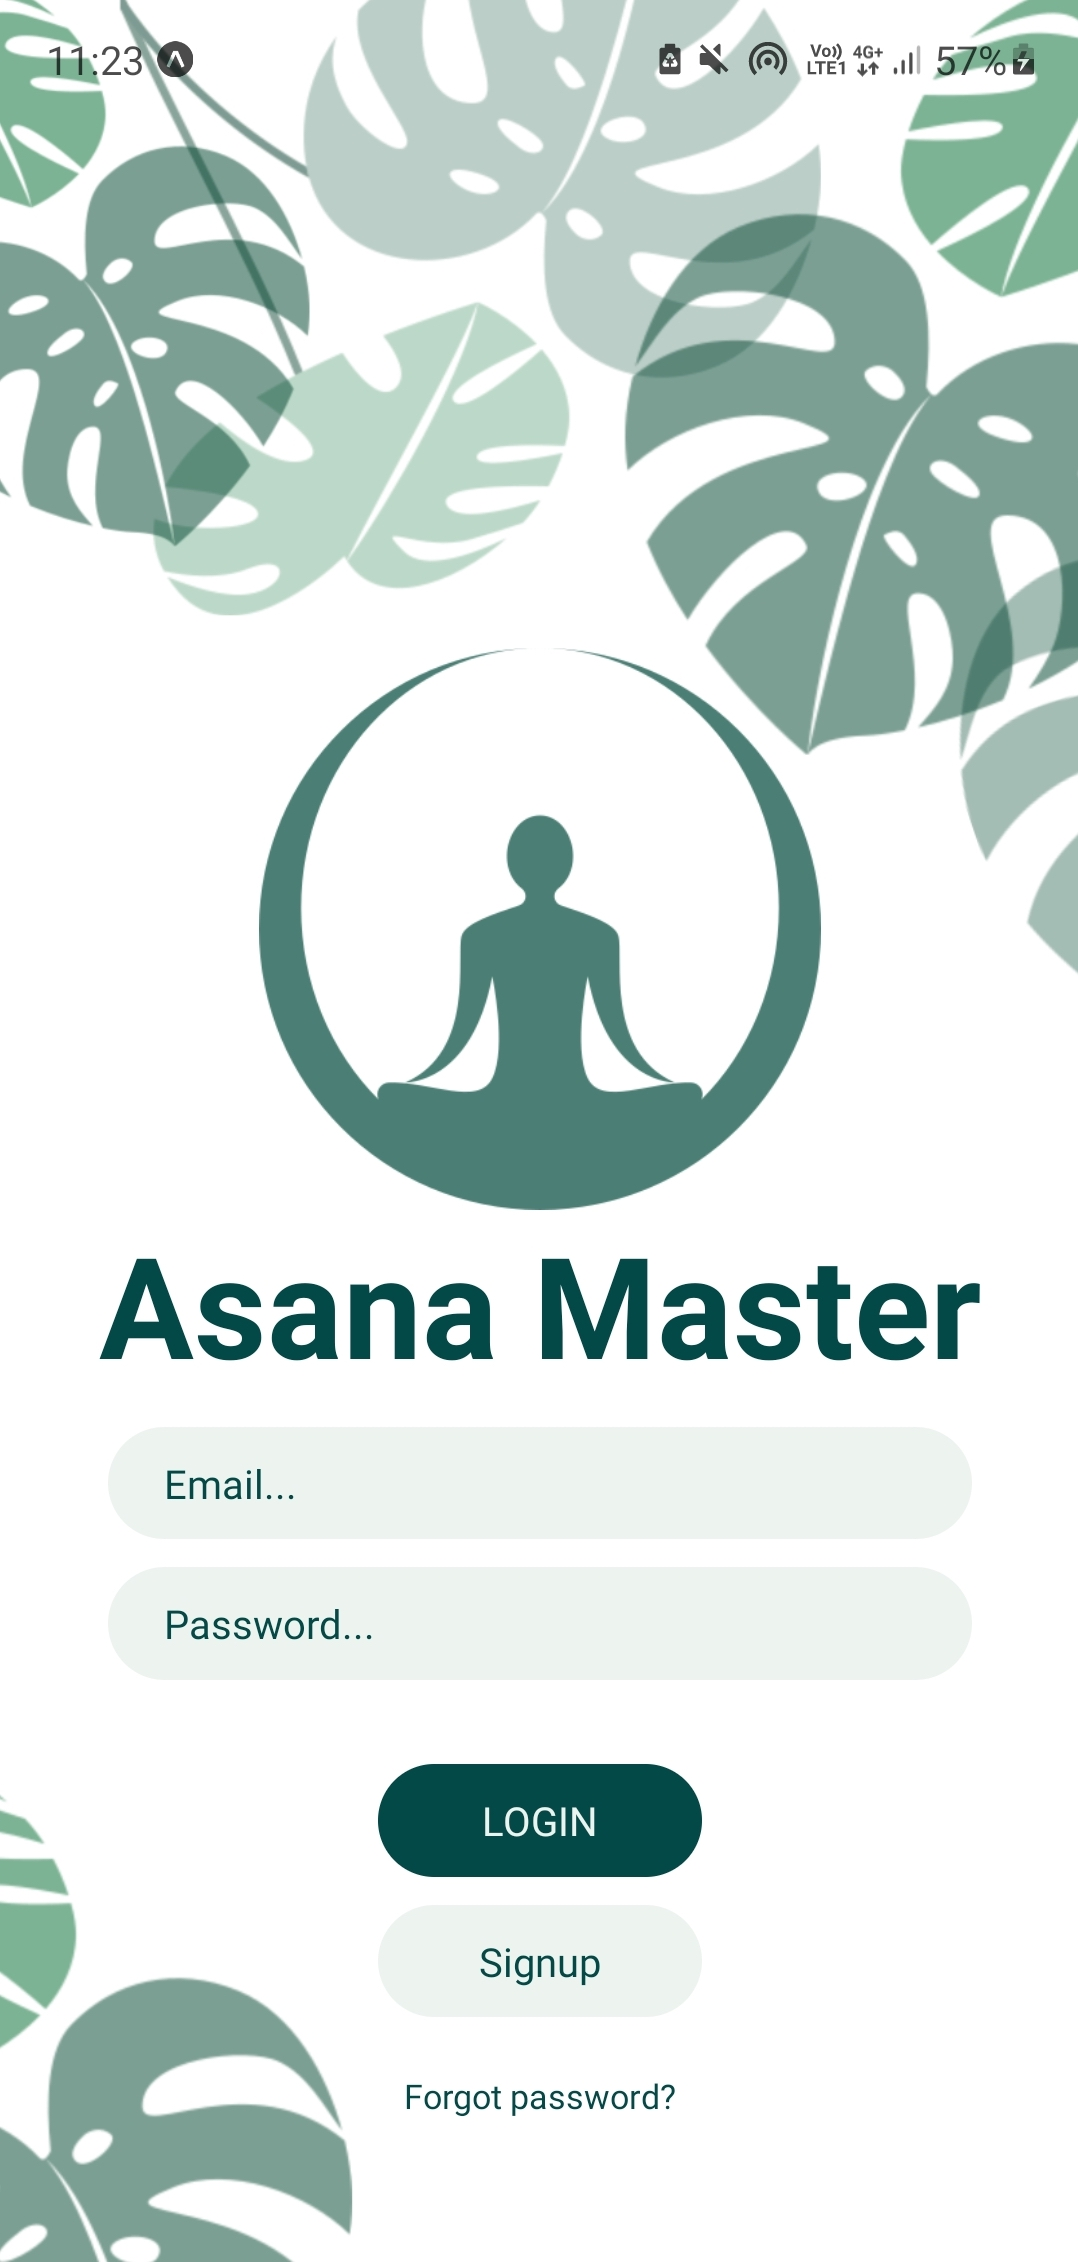
\includegraphics[width=\textwidth]{prijava.jpg}
    \caption{Prijavni obrazec ob vstopu v aplikacijo.}
    \label{prijava}
  \end{minipage}
  \begin{minipage}[b]{0.34\textwidth}
    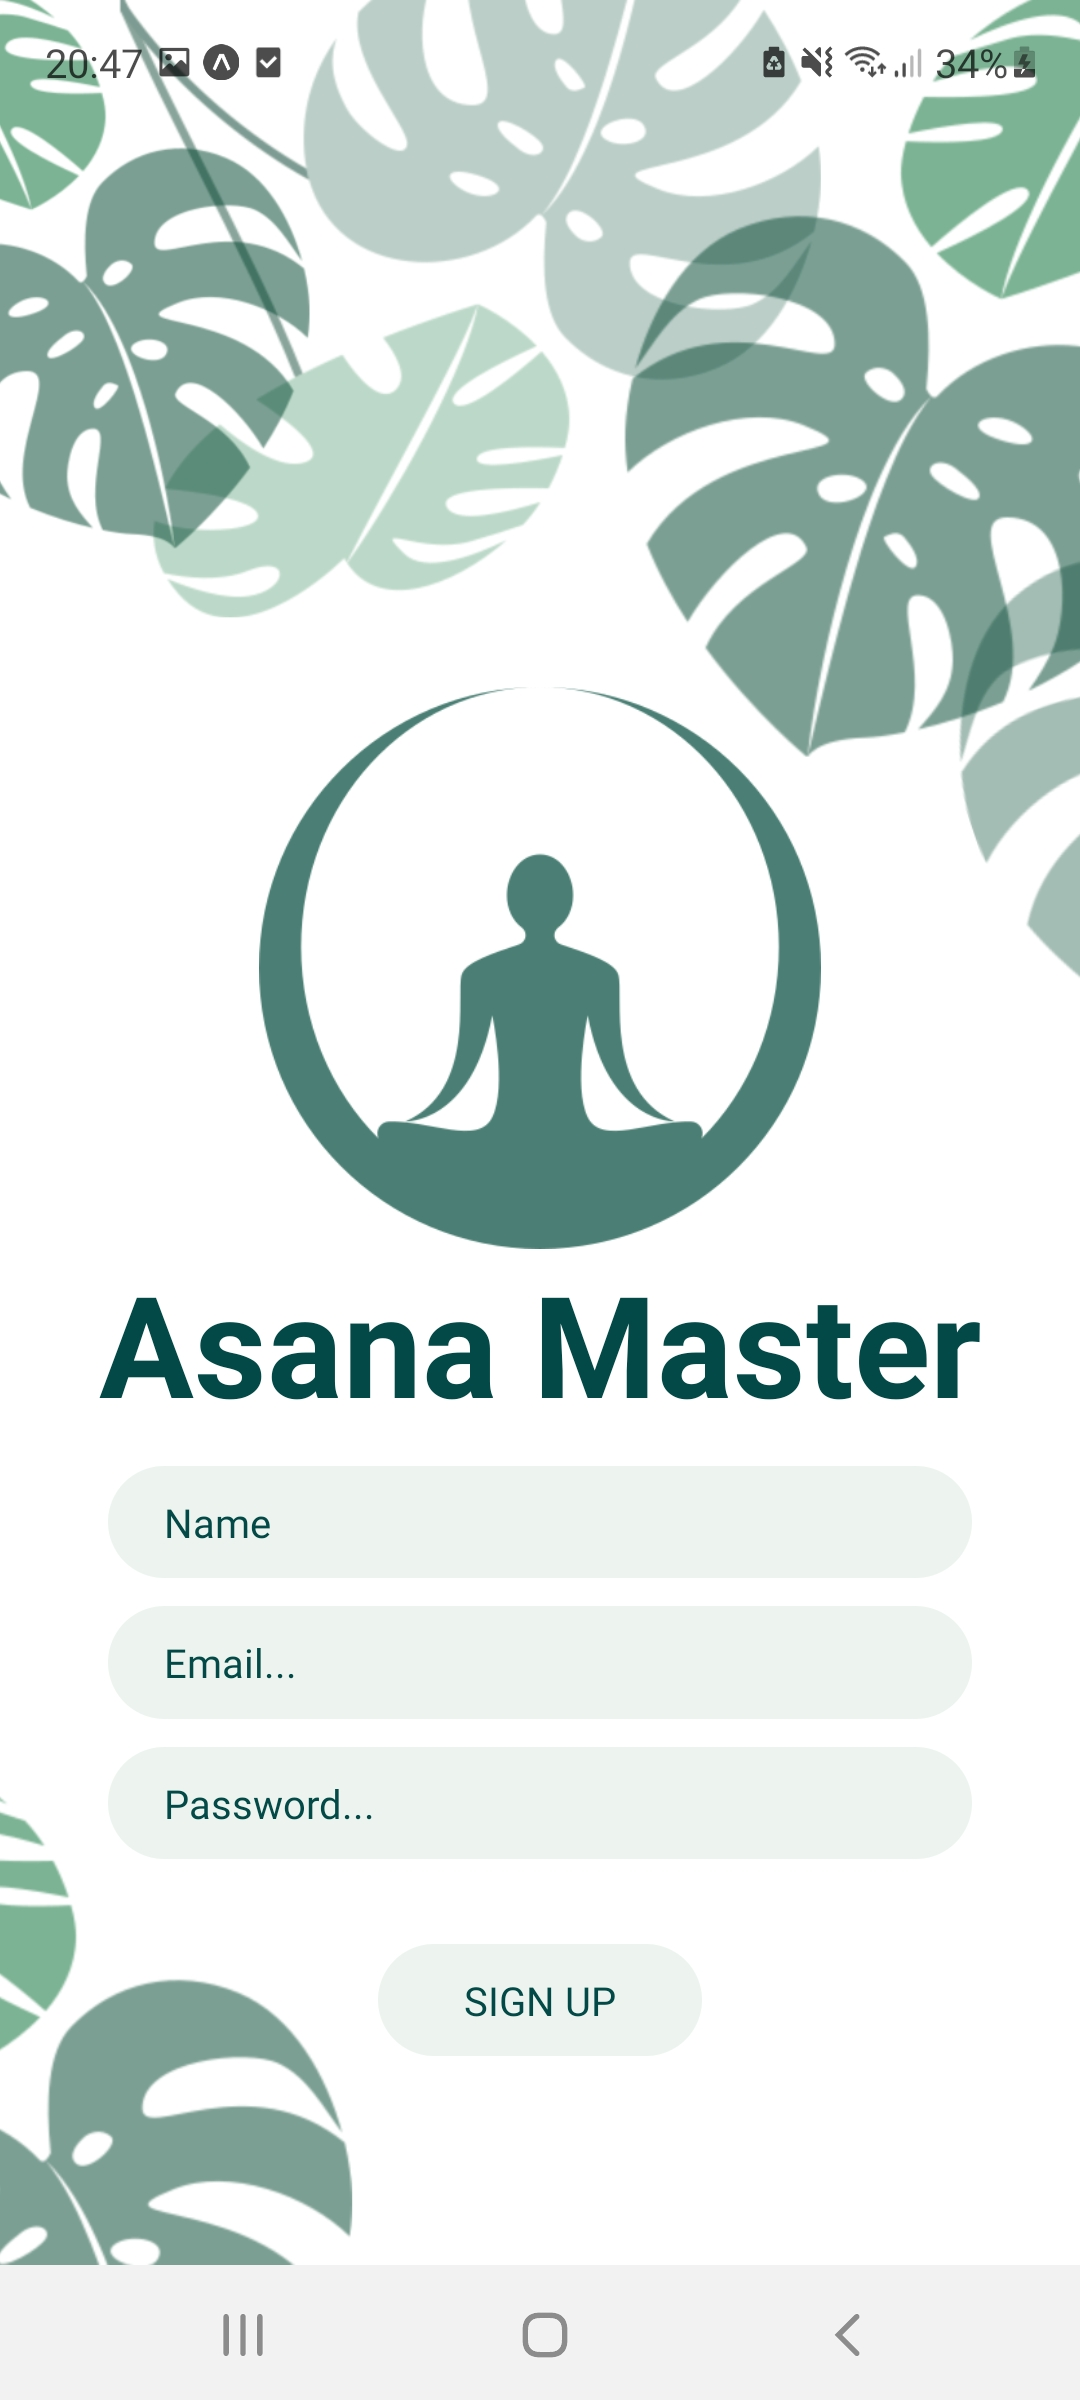
\includegraphics[width=\textwidth]{registracija.jpg}
    \caption{Obrazec za registracijo.}
	\label{registracija}
  \end{minipage}
  \begin{minipage}[b]{0.34\textwidth}
    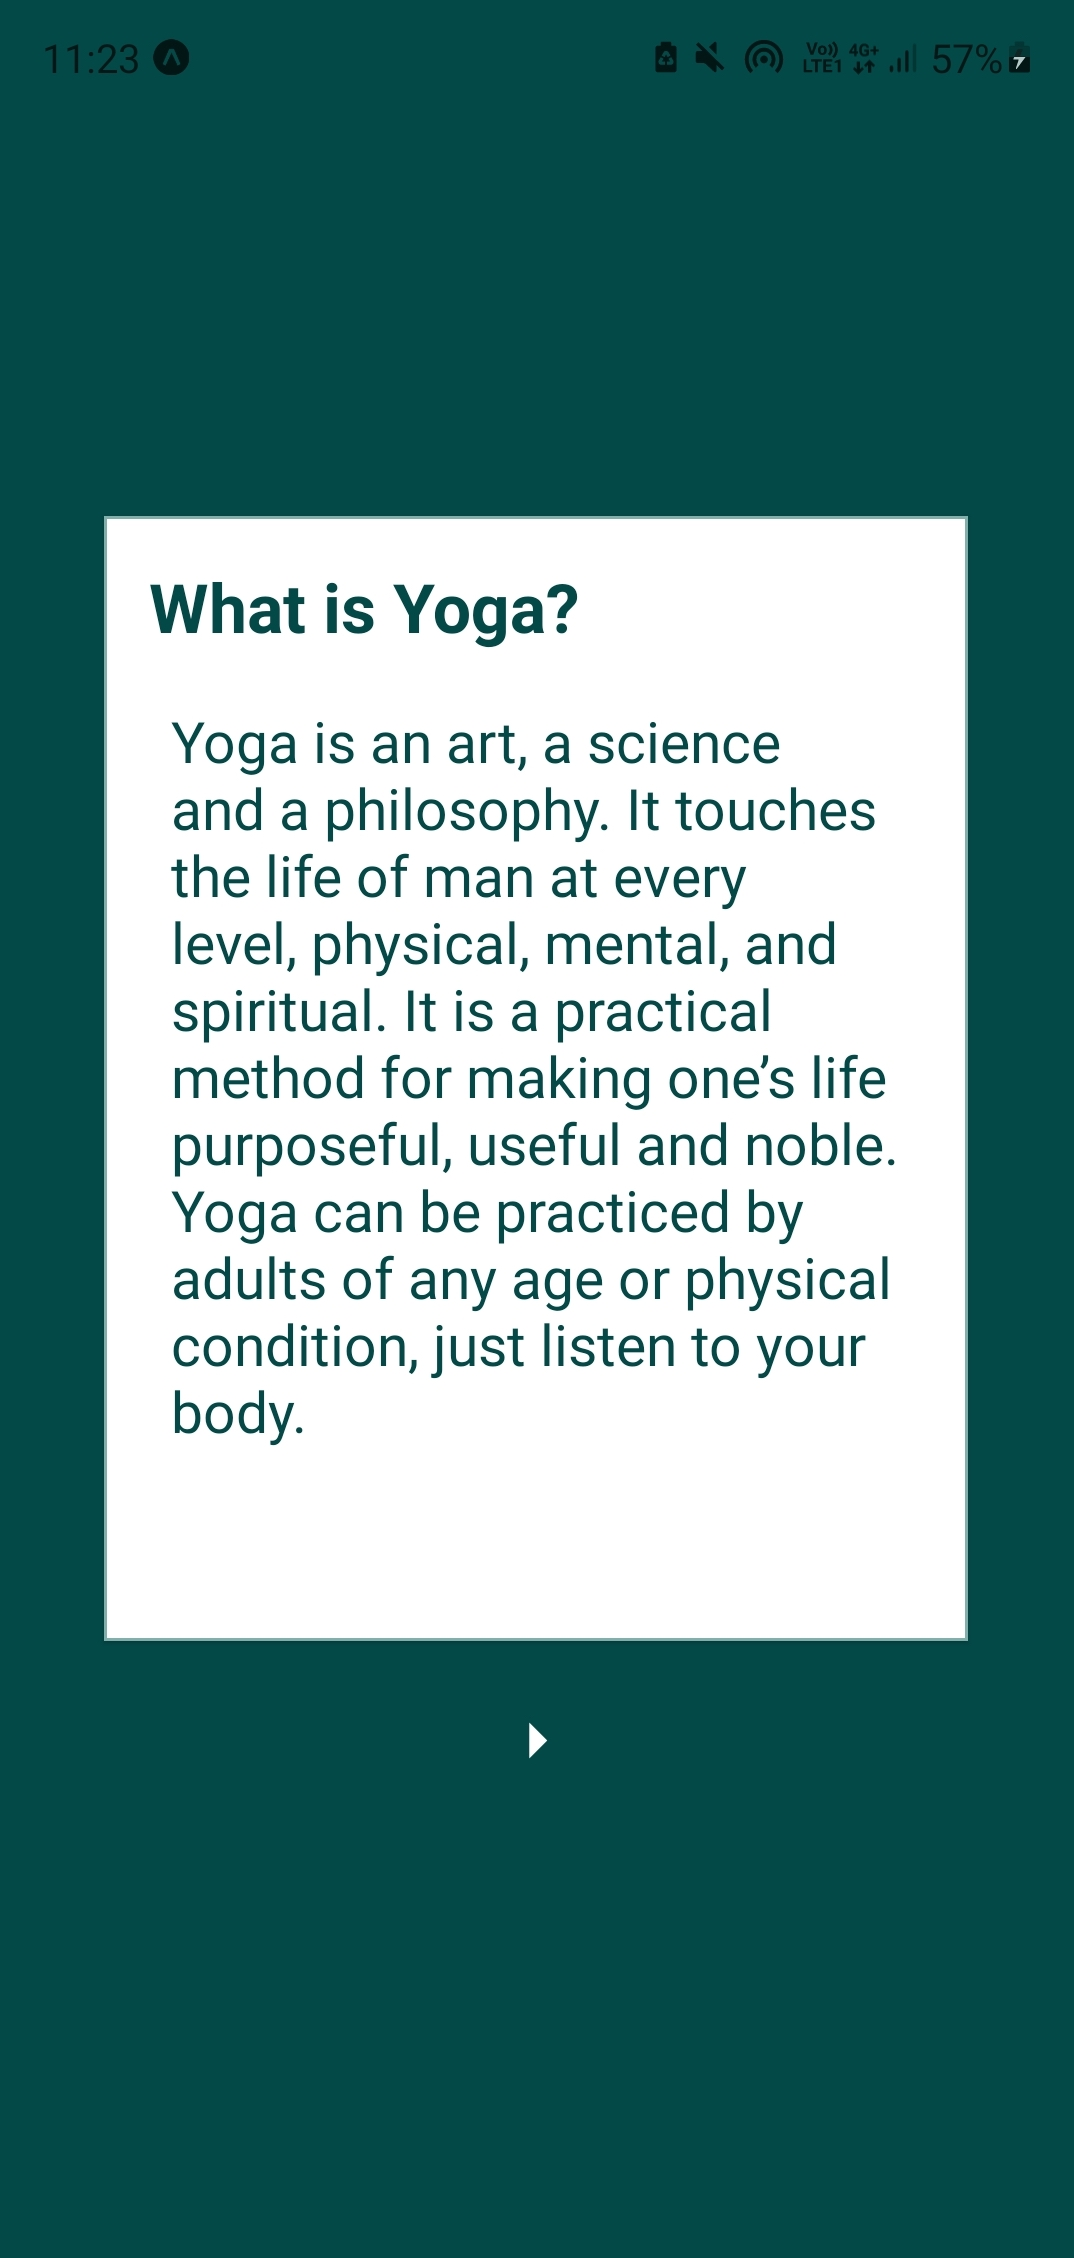
\includegraphics[width=\textwidth]{pozdrav1.jpg}
    \caption{Prijavni obrazec ob vstopu v aplikacijo.}
    \label{pozdrav1}
  \end{minipage}
  \begin{minipage}[b]{0.342\textwidth}
    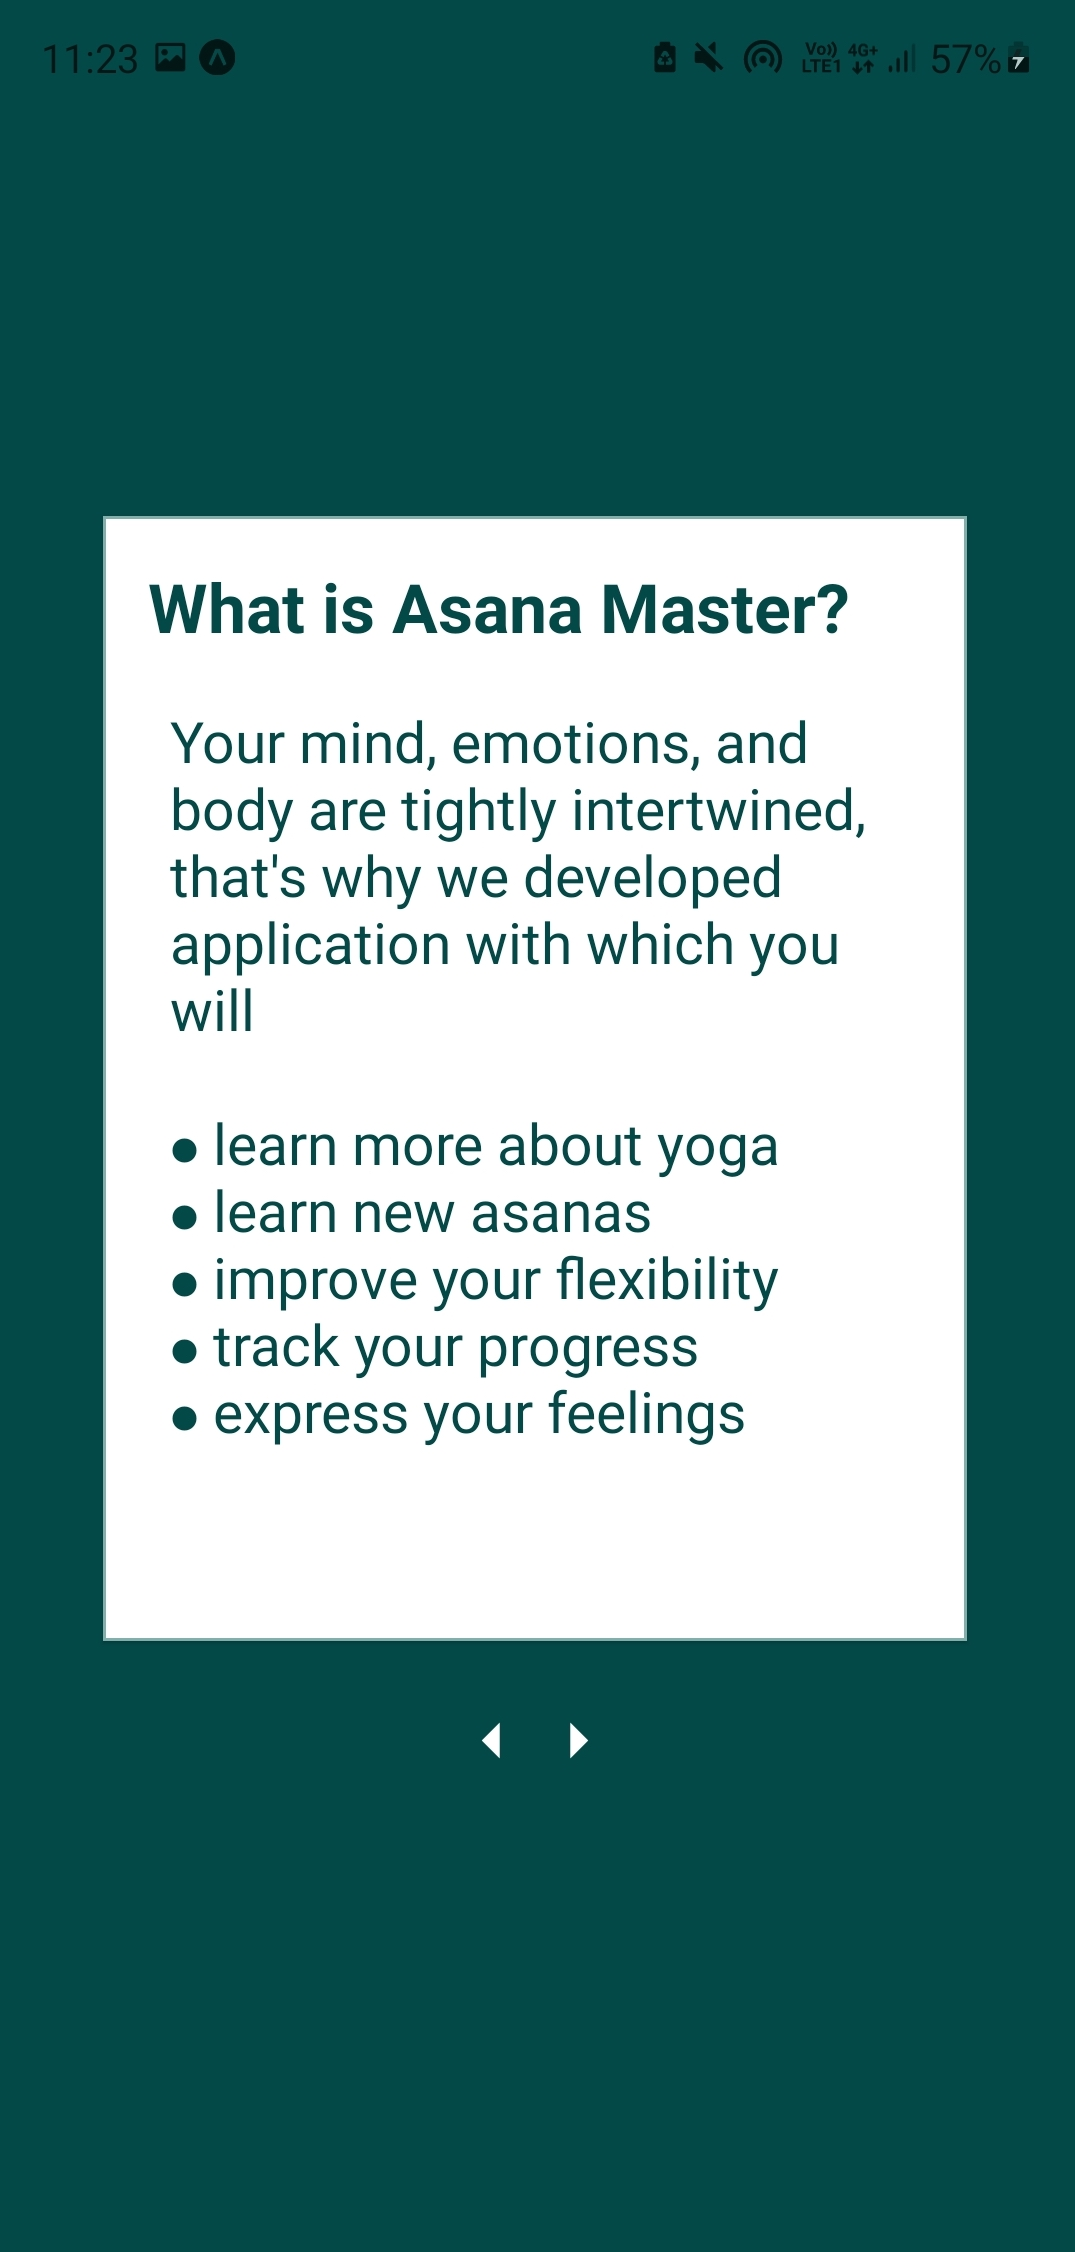
\includegraphics[width=\textwidth]{pozdrav2.jpg}
    \caption{Drugo pozdravno besedilo.}
	\label{pozdrav2}
  \end{minipage}
\end{figure}

Podmeni Asanas se razdeli še na 3 dodatne podstrani, ki določajo različne težavnosti položajev, to so Begginer, Intermediate in Master. V bazi podatkov imamo pri vsakem položaju shranjeno še njegovo stopnjo težavnosti, kar nam omogoča enostavno sortiranje v omenjene težavnosti. S klikom na eno izmed težavnosti se nam odpre seznam z imeni in slikami položajev. S klikom na določen položaj, pa se nam odpre stran z angleškim imenom, sanskrit imenom, sliko, opisom izvedbe in videoposnetkom položaja, (Slika~\ref{asana}). Uporabnik ima možnost ogleda videopostneka položaja, s klikom na posnetek. Vir videoposnetka je portal Youtube, posnetek pa se predvaja neposredno v sami aplikaciji, torej brez dodatnega odpiranja videoposnetka izven mobilne aplikacije. 

\begin{figure}[htbp]
\begin{center}
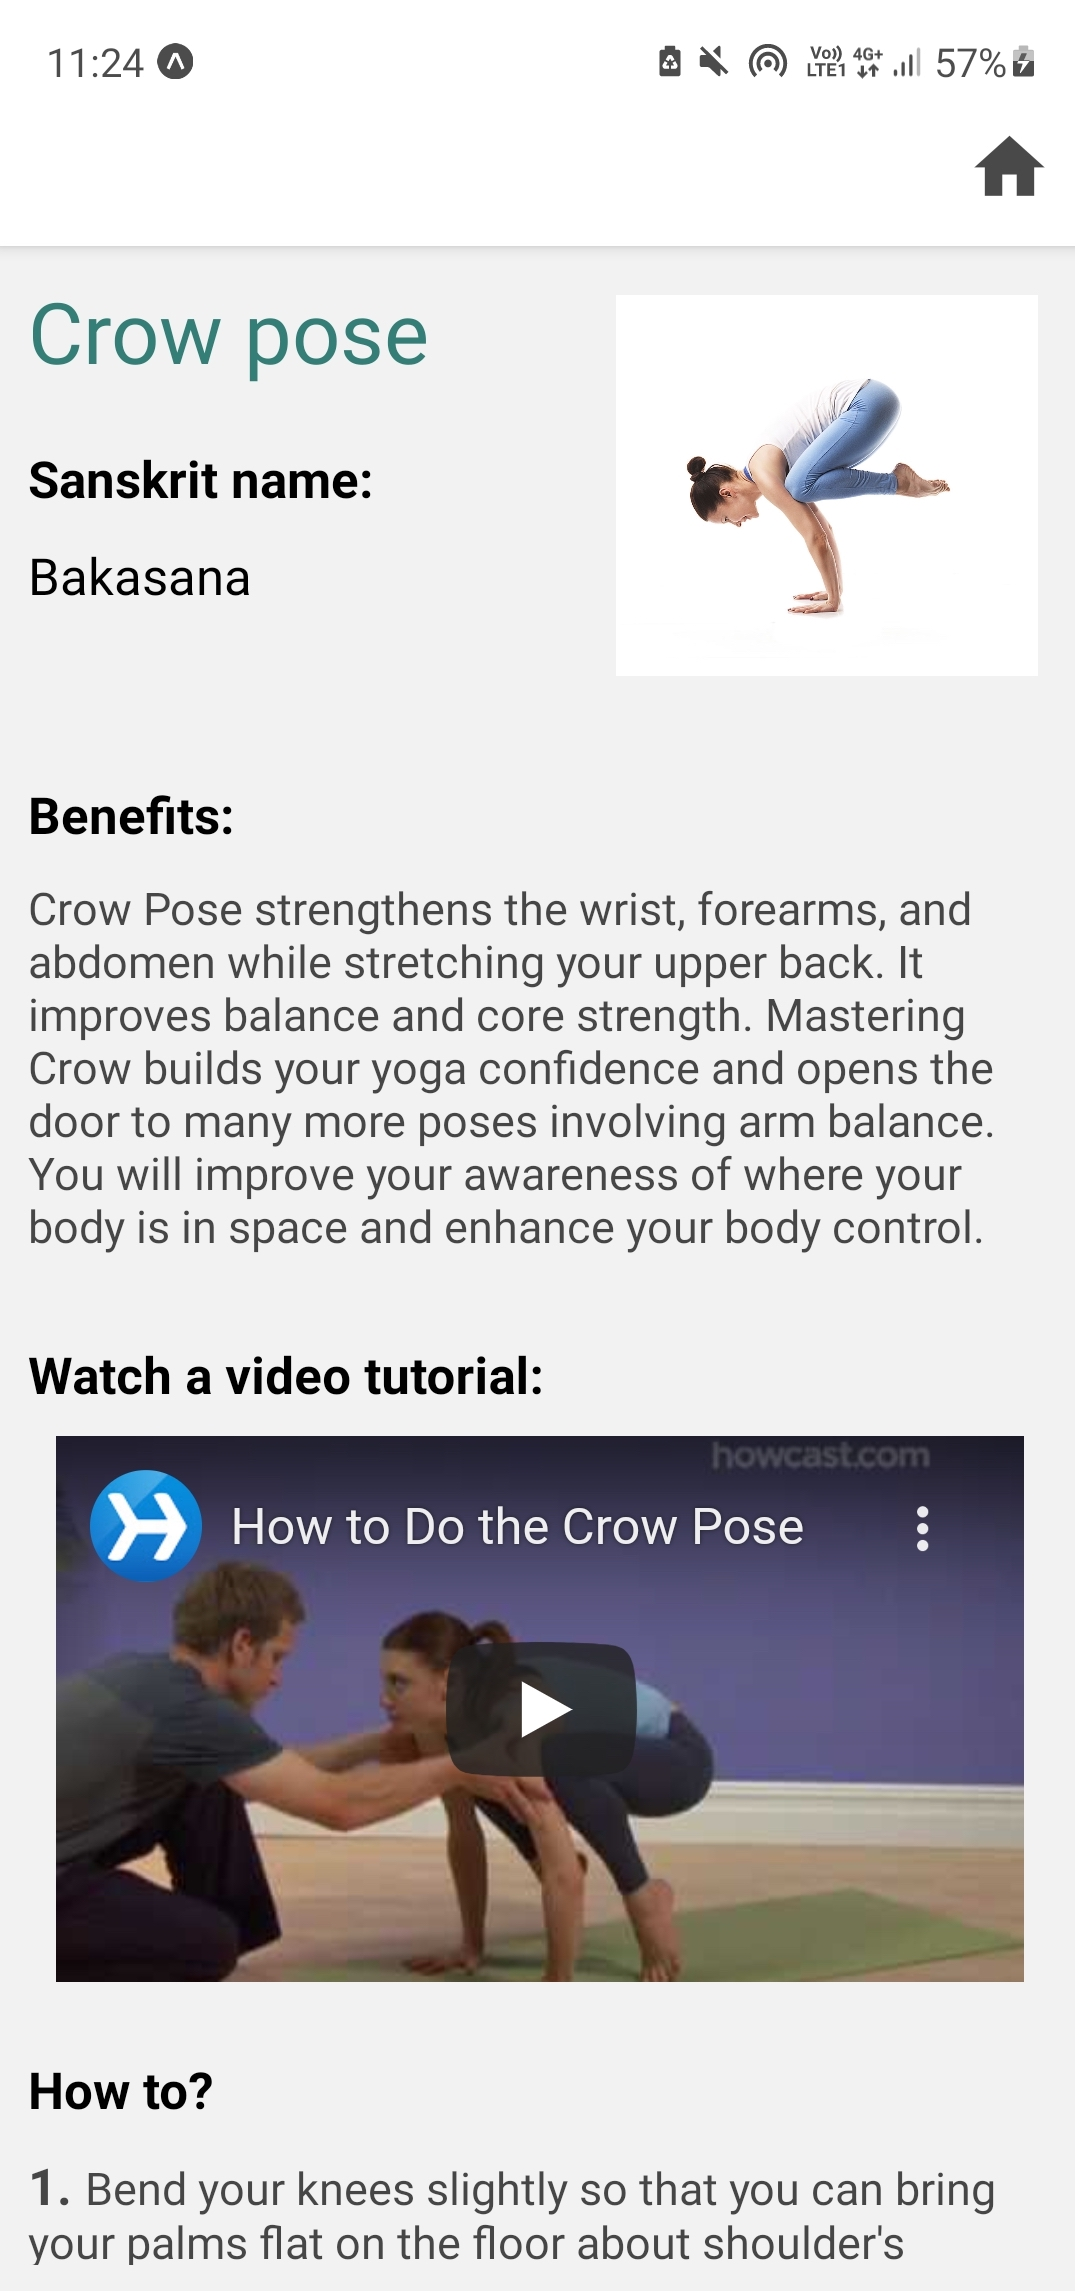
\includegraphics[scale=.14]{asana.jpg}
\end{center}
\caption{Stran s podrobnostmi o asani v podmeniju Asanas.}
\label{asana}
\end{figure}

Podmeni Goals se prav tako razdeli na 3 dodatne podstrani, ki predstavljajo 3 kategorije, v katerih se lahko uporabnik izboljša in spremlja svoj napredek. Kategorije so slednje, Splits, Backbends in Inversions. Ko si uporabnik izbere eno izmed kategorij, se odpre starn s 7 dnevnim programom različnih videoposnetkov, ki naj bi jim uporabnik sledil za lasten napredek. Prav tako kot pri položajih, smo tudi tukaj naredili tako, da uporabnik predvaja in odpre videoposnetek neposredno v aplikaciji, brez odpiranja novega okna izven aplikacije. 
Pod programom sledi še možnost dodajanja slik, s katerimi uporabnik lažje sledi napredku in pa možnosti samoocene, da si lahko lažje določi kje na poti do cilja se nahaja.\\

Podmeni Notes ima seznam zapiskov, ki jih je uporabnik ustvaril, ter spodaj desno gumb za dodajanje novega zapiska. S klikom na gumb za dodajanje zapiska, se uporabniku odpre forma za vnos naslova zapiska in okno za vnos vsebine zapiska. Spodaj pod oknom za vsebino pa se nahajata še 2 gumba, levo gumb Back, ki uporabnika vrne v seznam zapiskov in desno gumb Save, ki omogoča shranitev zapiska, (Slika~\ref{notes}). 

Zapisek, ki ga je uporabnik napisal in shranil, se v naslednjem koraku prikaže na seznamu zapiskov. Vsak zapisek v seznamu je prikazan z imenom na levi strani vrstice, na desni strani pa se nahaja gumb za izbris zapiska.
S klikom na zapisek se odpre stran z naslovom zapiska, datum, kdaj je bil zapisek ustvarjen in zapisano besedilo. \\


V glavnem meniju se v glavi nahaja gumb za odjavo, v vsakem podmeniju pa se v glavi nahaja gumb Home, ki omogoča vrnitev v glavni meni. 


\begin{figure}[htbp]
\begin{center}
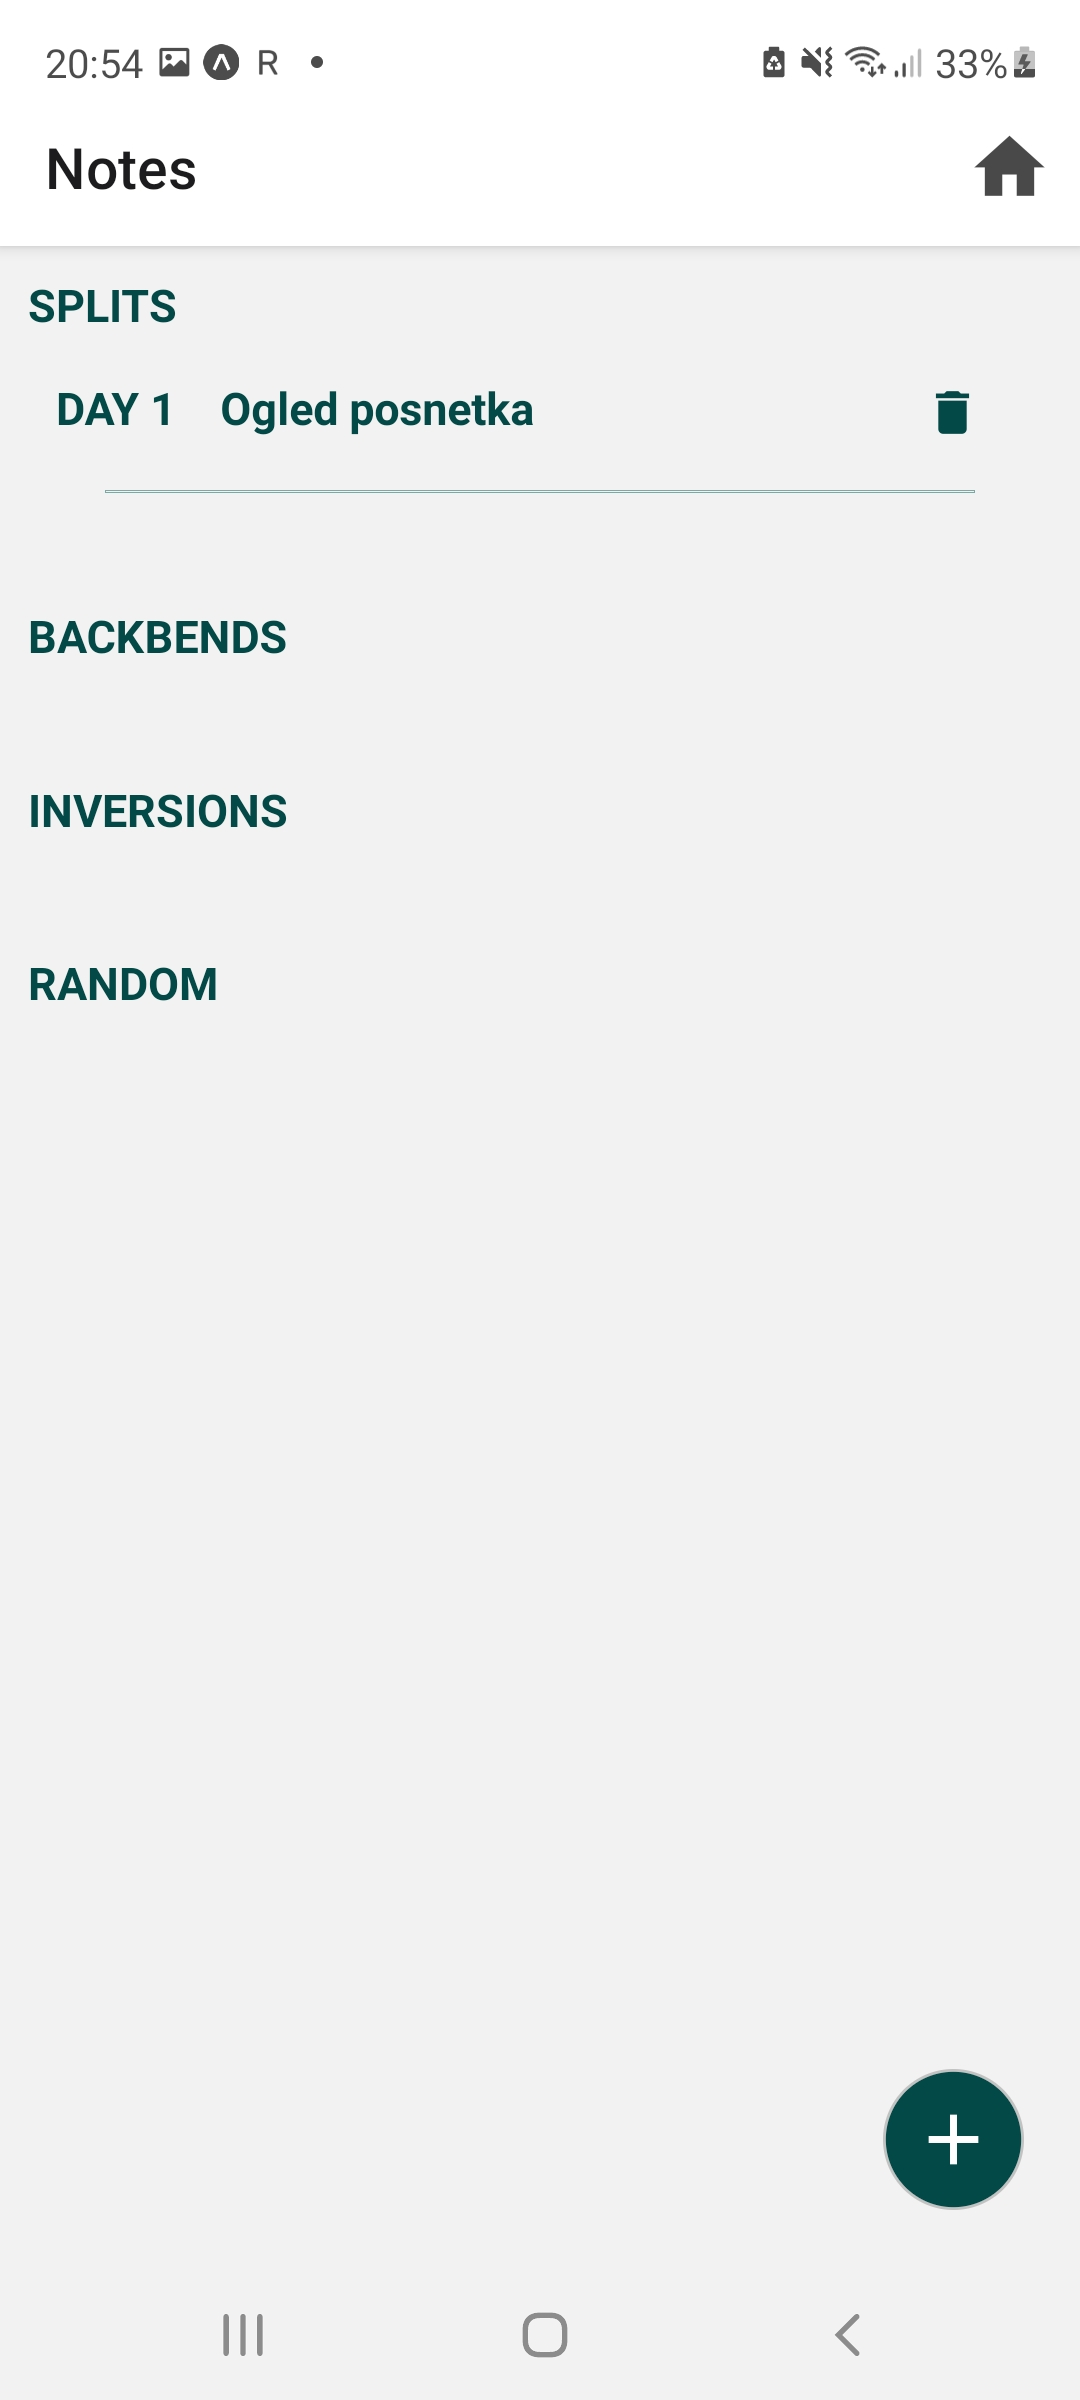
\includegraphics[scale=.2]{notes.jpg}
\end{center}
\caption{Stran za dodajanje novega zapiska, v podmeniju notes.}
\label{notes}
\end{figure}


\chapter{Tehnologije in orodja}
\label{ch2}

Mobilna aplikacija je razvita z uporabo ogrodja React Native in ogrodja Expo, kar omogoča izdelavo mobilnih aplikacij tako za operacijski sistem Android kot iOS. Za pisanje kode sta bila uporabljena jezika TypeScript in JavaScript. Koda aplikacije je bila napisana v programu Visual Studio Code. Za shranjevanje podatkov, ki so prikazani v aplikaciji, je uporabljena relacijska podatkovna baza MySql, ki je povezana z lokalnim strežnikom. 
Za testiranje aplikacije je bilo uporabljeno orodje React DevTools, ki omogoča enostavno testiranje aplikacij, tako na spletnem vmesniku, mobilnem simulatorju, kot tudi na mobilni napravi (Slika). Vse spremembe v kodi, ter zgodovina spremenjenih verzij aplikacije so shranjene v programu Git.

\includegraphics[scale=0.2]{../../../../../var/folders/k_/h6pfbkjd50lfxvygrngfcj900000gn/T/TemporaryItems/(A Document Being Saved By screencaptureui 16)/Screenshot 2021-07-16 at 11.50.09.png} 

\section{npm}
Npm je upravitelj paketov za platformo Node JavaScript. Namešča module, tako da jih vozlišče lahko najde, in inteligentno obvladuje konflikte med odvisnostmi. Izjemno prilagodljiv je za podporo najrazličnejšim primerom uporabe. Najpogosteje se uporablja za objavljanje, odkrivanje, nameščanje in razvoj vozliščnih programov.~\cite{npm}

\section{React Native}
React Native je JavaScript ogrodje za pisanje izvornih mobilnih aplikacij za operacijska sistema iOS in Android. Temelji na Reactu, Facebookovi JavaScript knjižnici za gradnjo uporabniških vmesnikov, a namesto na brskalnik cilja na mobilne platforme. 

React Native, je Facebook prvič izdal kot odprtokodni projekt leta 2015. V samo nekaj letih je postal ena najboljših rešitev za mobilni razvoj. React Native razvoj se uporablja za pogon nekaterih vodilnih svetovnih mobilnih aplikacij, vključno z Instagramom, Facebookom in Skypeom.~\cite{RN}

\section{Expo}
Expo je ogrodje, ki se uporablja za izdelavo React Native aplikacij. Gre za nabor orodij in storitev, zgrajenih okoli React Native-a in izvornih platform, ki nam pomagajo razvijati, graditi, uvajati in hitro iterirati v iOS, Android in spletne aplikacije iz iste kodne baze JavaScript / TypeScript. Z uporabo Expo-ta ne potrebujemo znanja o izvorni iOS ali Android kodi, kar pomeni, da tudi uporaba orodij kot sta Xcode ali Android Studio, ni potrebna. Njegov cilj je omogočiti hiter razvoj, ne da bi morali veliko časa porabiti za vzpostavljanje razvojnega okolja. Expo ne zahteva nastavitve IDE-jev, specifičnih za platforme, kot je to v primeru React Native CLI, in ke zato celoten postopek namestitve veliko bolj enostaven.~\cite{EXPO}

\section{JavaScript}
JavaScript (krajše tudi JS) je skriptni programski jezik, katerega je razvil Netscape, da bi bil v pomoč programerjem pri izdelavi spletnih strani. Večina tistih, ki pozna vsaj nekaj osnov programiranja, ko zasliši ime JavaScript, hitro poveže s programskim jezikom Java, s katerim imata kar nekaj skupnih lastnosti. Na splošno velja, da so skriptni jeziki enostavnejši in hitrejši v primerjavi s kodo v bolj kompleksnih programskih jezikih kot C in C++. Pri skriptnih jezikih v splošnem obdelava kode traja dalje kot pri zbirnih jezikih, vendar pa so veliko bolj uporabni pri krajših programih zaradi njihove enostavnosti. Uporabnost JavaScript-a pride najbolj do izraza pri razvoju dinamičnih spletnih strani in dodajanju interaktivnosti na želeno stran.

https://www.theserverside.com/definition/JavaScript

\section{TypeScript}
TypeScript je odprtokodni jezik, ki temelji na JavaScriptu, enem izmed najbolj uporabljenih jezikov na svetu, z dodajanjem statičnih definicij tipa. Tipi nam ponujajo način za opis oblike predmeta, zagotavljajo boljšo dokumentacijo in omogočajo TypeScriptu, da preveri, ali koda deluje pravilno.

Vsa veljavna koda napisana v jeziku JavaScript je tudi koda TypeScript. TypeScript se prek prevajalnika TypeScript ali Babel pretvori v JavaScript. JavaScript koda je čista in preprosta in se izvaja kjerkoli, kjer deluje JavaScript: v brskalniku, na Node.JS ali v aplikacijah.https://www.typescriptlang.org/

\section{Visual Studio Code}
Za pisanje kode je bil uporabljen program Visual Studio Code, znan tudi kot VS Code, ki je Microsoftov brezplačen odprtokodni urejevalnik besedil. VS Code je na voljo za Windows, Linux in macOS. Čeprav je urejevalnik razmeroma lahek, vključuje nekaj zmogljivih funkcij, zaradi katerih je VS Code v zadnjem času postalo eno najbolj priljubljenih orodij za razvojno okolje.

\section{MySQL}
Prilagodljiv in zmogljiv program, MySQL je najbolj priljubljen odprtokodni sistem zbirk podatkov na svetu. Kot del široko uporabljenega svežnja tehnologij LAMP (ki ga sestavljajo operacijski sistem, ki temelji na Linuxu, spletni strežnik Apache, baza podatkov MySQL in PHP za obdelavo) se uporablja za shranjevanje in pridobivanje podatkov v najrazličnejših priljubljenih aplikacijah. , spletna mesta in storitve.
https://www.digitalocean.com/community/tutorials/what-is-mysql

\section{TablePlus}
Za pregledovanje in urejanje baze podatkov je bil uporabljen program TablePlus. TablePlus je sodobna, izvorna aplikacija s čistim uporabniškim vmesnikom, ki razvijalcem omogoča sočasno upravljanje podatkovnih baz na zelo hiter in varen način. TablePlus podpira večino priljubljenih baz podatkov, kot so MySQL, Postgres, SQL Server, SQLite, Microsoft SQL Server, Redis, Redshift, Oracle in še veliko več.
https://mariadb.com/kb/en/tableplus/

\section{Git}
Git je brezplačen in odprtokodni porazdeljeni sistem za nadzor različic, zasnovan za hitro in učinkovito obdelavo vsega, od majhnih do zelo velikih projektov.
https://git-scm.com/



\chapter{Testno okolje}
\label{ch3}



\chapter{Prototip aplikacije}
\label{ch4}


\chapter{Zaključek}
\label{stroka}


\clearpage
\addcontentsline{toc}{chapter}{Literatura}
\bibliographystyle{plain}
\bibliography{literatura}

\end{document}

